% +------------------------------------------------------------------------+
% | Skin_surface_3/doc_tex/Skin_surface_3/main.tex
% +------------------------------------------------------------------------+
% | Meshing the 3d Skin surface defined for a set of spheres.
% | 
\RCSdef{\skinSurfaceRev}{$Id$}
\RCSdefDate{\skinSurfaceDate}{$Date$}
% +------------------------------------------------------------------------+

\newcommand{\dabs}[1]{{\parallel\! #1 \!\parallel}}

\ccUserChapter{3D Skin Surface Meshing}
\label{chapter_SkinSurface}
\ccChapterRelease{\skinSurfaceRev. \ \skinSurfaceDate}
\ccChapterAuthor{Nico Kruithof}

\minitoc

\begin{ccTexOnly}
\begin{center}
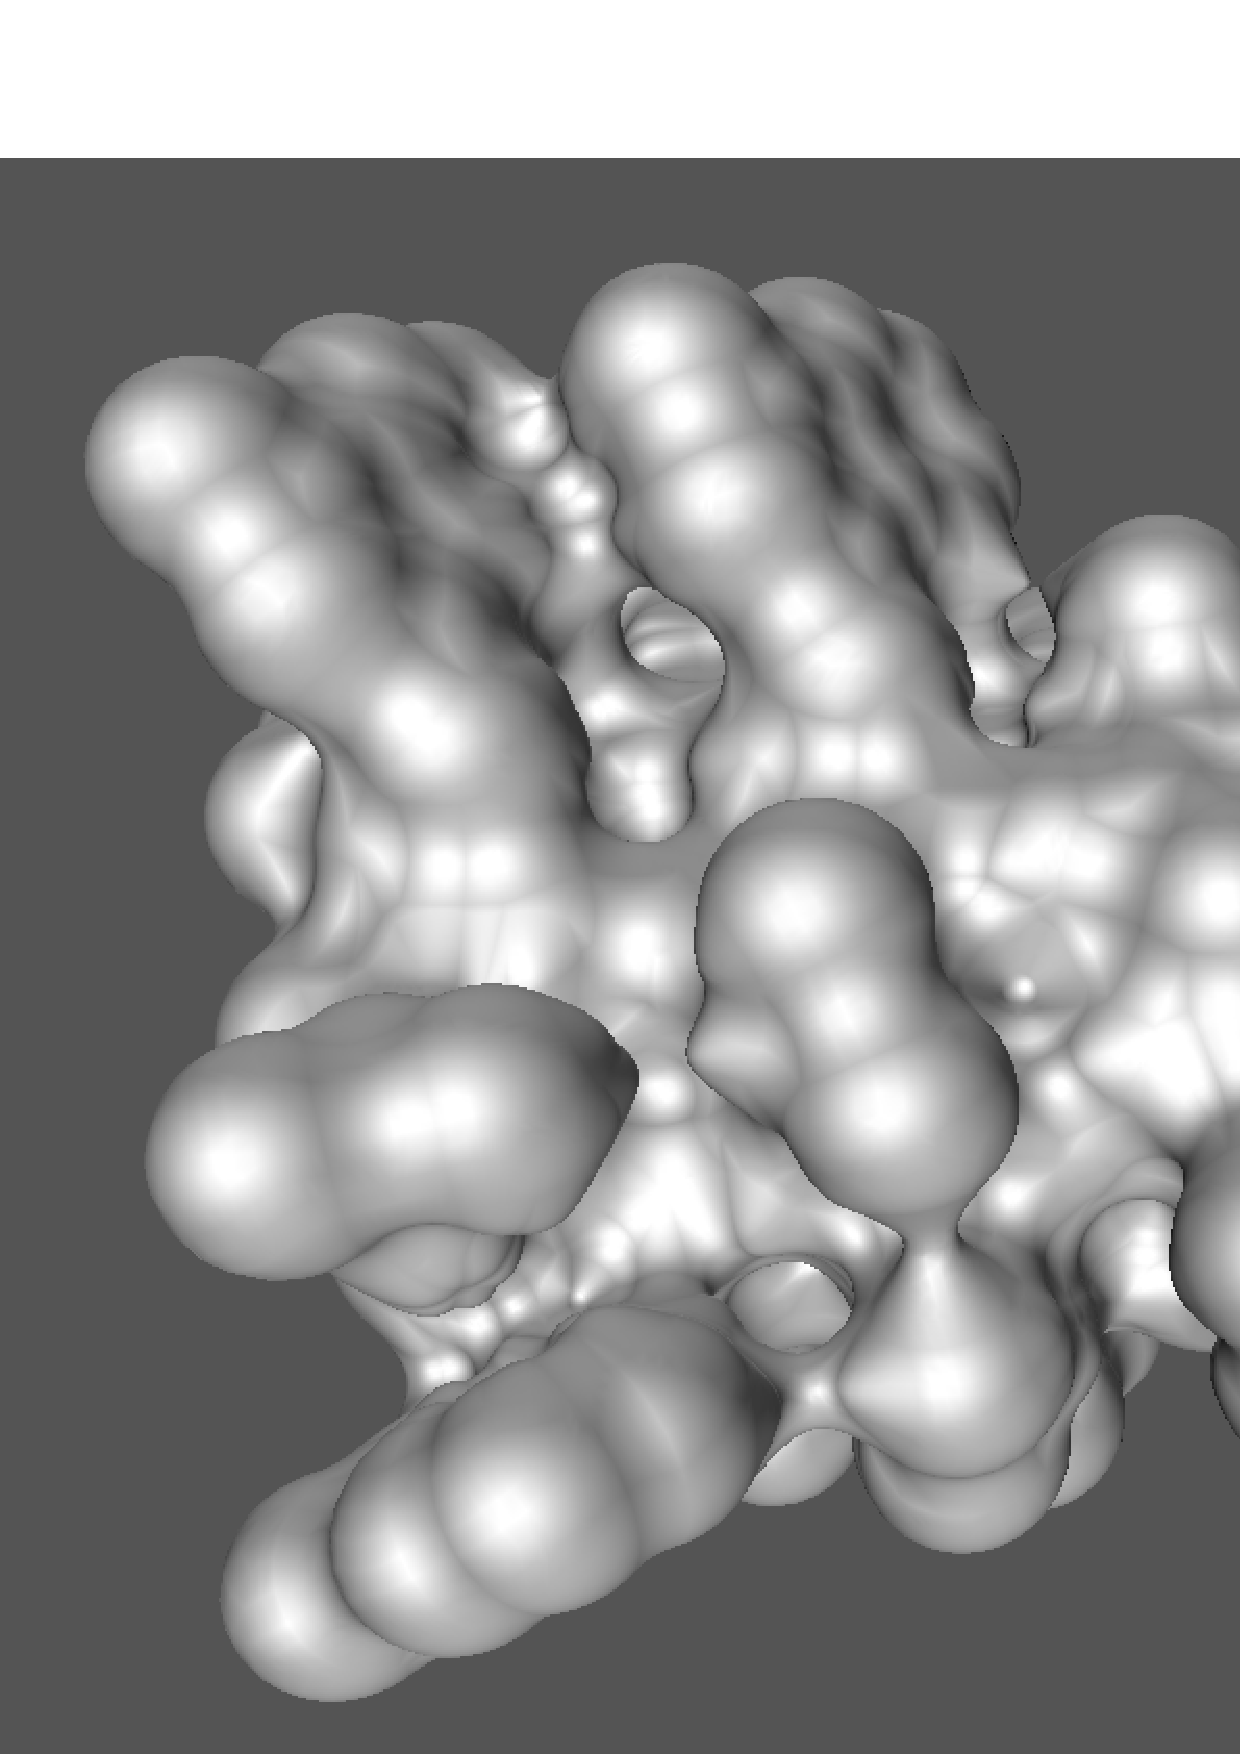
\includegraphics[width=.9\textwidth]{Skin_surface_3/molecule}
\end{center}
\end{ccTexOnly}
\begin{ccHtmlOnly}
<img border="0" src="./molecule.png" align="center" height="75%">
\end{ccHtmlOnly}

% +------------------------------------------------------------------------+
\section{Introduction}
\label{sectionSkinSurfaceIntro}

Skin surfaces, introduced by Edelsbrunner in \cite{cgal:e-dssd-99},
have a rich and simple combinatorial and geometric structure that
makes them suitable for modeling large molecules in biological
computing.  Meshing such surfaces is often required for further
processing of their geometry, like in numerical simulation and
visualization.

A skin surface is defined by a set of weighted points (input balls)
and a scalar called the shrink factor. If the shrink factor is equal
to one, the surface is just the boundary of the union of the input
balls.  If the shrink factor decreases, the skin surface becomes
tangent continuous, due to the appearance of patches of spheres and
hyperboloids connecting the balls.

This package constructs an isotopic mesh from a set of balls and a
shrink factor using the algorithm described in
\cite{cgal:kv-mssct-05}. It also provides an interface to the surface
mesher presented in Chapter~\ref{chapter_SurfaceMesher} by providing a
model of the concept \ccc{SurfaceMeshTraits_3}.
%An optimized algorithm is implemented for meshing the union of a set of balls.

\section{Definition of a skin surface}
\label{sec:skindefinition}

\begin{figure}
  \begin{ccTexOnly}
    \begin{center}
      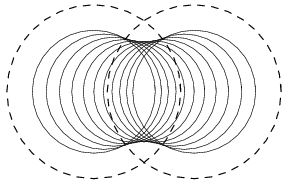
\includegraphics[width=.25\textwidth]{Skin_surface_3/skinTwoPoints}
    \end{center}
  \end{ccTexOnly}
  \begin{ccHtmlOnly}
    <img border="0" src="./skinTwoPoints.png" align="center" alt="Skin
    curve of two weighted points">
  \end{ccHtmlOnly}
  \caption{\label{fig:twoPoints} The skin curve of two weighted points
    (the two dashed circles). The smaller circles form a subset of the
    shrunk convex hull of the input points. Its boundary forms the skin
    curve. }
\end{figure}

This section first briefly reviews skin surfaces. For a more thorough
introduction to skin surfaces, we refer to \cite{cgal:e-dssd-99} where
they were originally introduced.

A skin surface is defined in terms of a finite set of weighted points
$\hat{P}$ and a shrink factor $s$, with $0\leq s\leq 1$. A weighted
point $\hat{p}=({p},\textsc{p})\in \R^d\times\R$ corresponds to a ball
with center ${p}$ and radius $\sqrt{\textsc{p}}$. If $\textsc{p}<0$,
then the weighted point corresponds to an imaginary ball (a ball with
imaginary radius).

The space of weighted points inherits a vector space structure from
$\R^{d+1}$ via the bijective map
$\Pi:\R^d\!\times\!\R\mapsto\R^{d+1}$, defined by 
%
\[
\Pi(\hat{p}) = (x_1,\ldots,x_d,\dabs{{p}}^2-\textsc{p}),
\]
%
with ${p}=(x_1,\ldots,x_d)$. Addition of two weighted points and the
multiplication of a weighted point by a scalar are defined in the
vector space structure inherited under $\Pi$. For further reading on
the space of circles and spheres we refer to \cite{p-gcc-70}.

Starting from a weighted point $\hat{p}=({p},\textsc{P})$, the
shrunk weighted point $\hat{p}^s$ is defined as $\hat{p}^s =
({p},s\cdot \textsc{p})$.  The set $\hat{P}^s$ is the set
obtained by shrinking every weighted point of $\hat{P}$ by a
factor $s$.

The skin surface $\mbox{skn}^{s}(\hat{P})$ and its body
$\mbox{bdy}^{s}(\hat{P})$ associated with a set of weighted points
$\hat{P}$, are defined by
\begin{eqnarray}
  \label{eq:defbody}
  \mbox{bdy}^{s}(\hat{P}) &=& \cup(\mbox{conv} (\hat{P}))^s\\
  \label{eq:defskin}
  \mbox{skn}^{s}(\hat{P}) &=& \partial{\mbox{bdy}^{s}(\hat{P})}.
\end{eqnarray}
%
Here $\mbox{conv}(\hat{P}) \subset \R^d\times\R$ is the convex hull --
with respect to the vector space structure inherited under $\Pi$ -- of
a set of weighted points $\hat{P}$, whereas $\partial$ denotes the
boundary -- in $\R^d$ -- of the union of the corresponding set of
balls. For a skin curve in $2D$ associated with two weighted points:
see Figure~\ref{fig:twoPoints}.

%There exists a polyhedral complex that decomposes a skin surface into
%pieces quadrics. 

\section{The interface}
The interface to the skin surface package consists of three distinct
global functions and a class \ccc{Skin_surface_3} which is a model of
the concept \ccc{Surface_3}.  The first function takes a list of
weighted points and a shrink factor and outputs a
\ccc{Skin_surface_3}. It has two overloaded functions:

\ccGlobalFunction{template <class Iterator,
                            class FT,
                            class SkinSurface_3>
void make_skin_surface_3
(Iterator begin,
 Iterator end,
 FT shrinkfactor,
 SkinSurface_3 skin_surface) ;}
\ccGlobalFunction{template <class Iterator,
                            class FT,
                            class SkinSurface_3,
                            class SkinSurfaceTraits_3>
void make_skin_surface_3
(Iterator begin,
 Iterator end,
 FT shrinkfactor,
 SkinSurface_3 skin_surface,
 SkinSurfaceTraits_3 traits) ;}

With the \ccc{SkinSurface_3} object it is possible to generate a
coarse mesh isotopic to the skin surface. 

\ccGlobalFunction{template <class SkinSurface_3,
                            class FT,
                            class Polyhedron>
void mesh_skin_surface_3
(SkinSurface_3 skin_surface,
 Polyhedron &p) ;}

The last function takes the (coarse) mesh and subdivides it in-situ by
applying a given number of 1-4 split operations (each triangle is
split into four sub-triangles) and then moving the vertices on the
skin surface. A model of the \ccc{SkinSurface_3} object is needed to
move the new points on the skin surface.

\ccGlobalFunction{template <class Polyhedron,
                            class SkinSurface_3 >
void subdivide_skin_surface_mesh_3 
(Polyhedron &p,
 SkinSurface_3 &skinsurface,
 int iterations);}
%
The class \ccc{Skin_surface_3} is both a model of the concept
\ccc{SkinSurface_3} and the concept \ccc{Surface_3}.
Therefore it can be used in the surface mesher described in
Chapter~\ref{chapter_SurfaceMesher}.

\section{Timings}
The timings of the construction of the coarse mesh and the first
subdivision are given in seconds.
\begin{center}
  \begin{tabular}{|l|c|c|c|}
    \hline
    Dataset & Number of weighted points & Coarse mesh & first subdivision step\\
    \hline
    \hline
    Caffeine& 23 & 0.2 & 0.05 \\
    Gramicidin A& 318 & 5 & 2\\
    \hline
  \end{tabular}
\end{center}
The timings were done on a Pentium 4, 3.5 GHz, with 1 Gb of memory.
\section{Example programs}
\subsection{Meshing a skin surface}
The following example shows the construction of a coarse mesh of the
skin surface from an iterator range of weighted points and a shrink factor.
\ccIncludeExampleCode{Skin_surface_3/skin_surface_simple.C}

\subsection{Meshing and subdividing a skin surface}
This example extends the previous examples with a subdivision of the
coarse mesh to obtain a better approximation. The extension of the
polyhedron is not necessary, but gives a significant speedup.
\ccIncludeExampleCode{Skin_surface_3/skin_surface_sqrt3.C}



\section{Marching tetrahedra}
The marching tetrahedra algorithm, introduced in
\cite{cgal:tpg-rmtiise-99}, is used in the construction of the coarse
mesh isotopic to skin surface. This algorithm is of general use and
therefore also documented.

The marching tetrahedra algorithm extracts a mesh from a
triangulation.  First, it labels each vertex of the triangulation
either as inside or as outside. The vertices of the mesh are
constructed as the intersection point of the surface and an edge with
different vertex-labels. The faces of the mesh are defined by the
tetrahedra of the triangulation. Based on the number of
triangulation-vertices inside the surface, we can distinguish five
cases, two of which are redundant if we allow the exchange of inside
and outside. In the case that all four labels are equal, the
tetrahedron does not contain a part of the surface. If three labels
are equal, the three vertices of the mesh form a triangle. If two
labels are equal, we construct two triangles. These three cases are
depicted in Figure~\ref{SkinSurface3-fig-marching}.

\begin{figure}
\begin{ccTexOnly}
\begin{center}
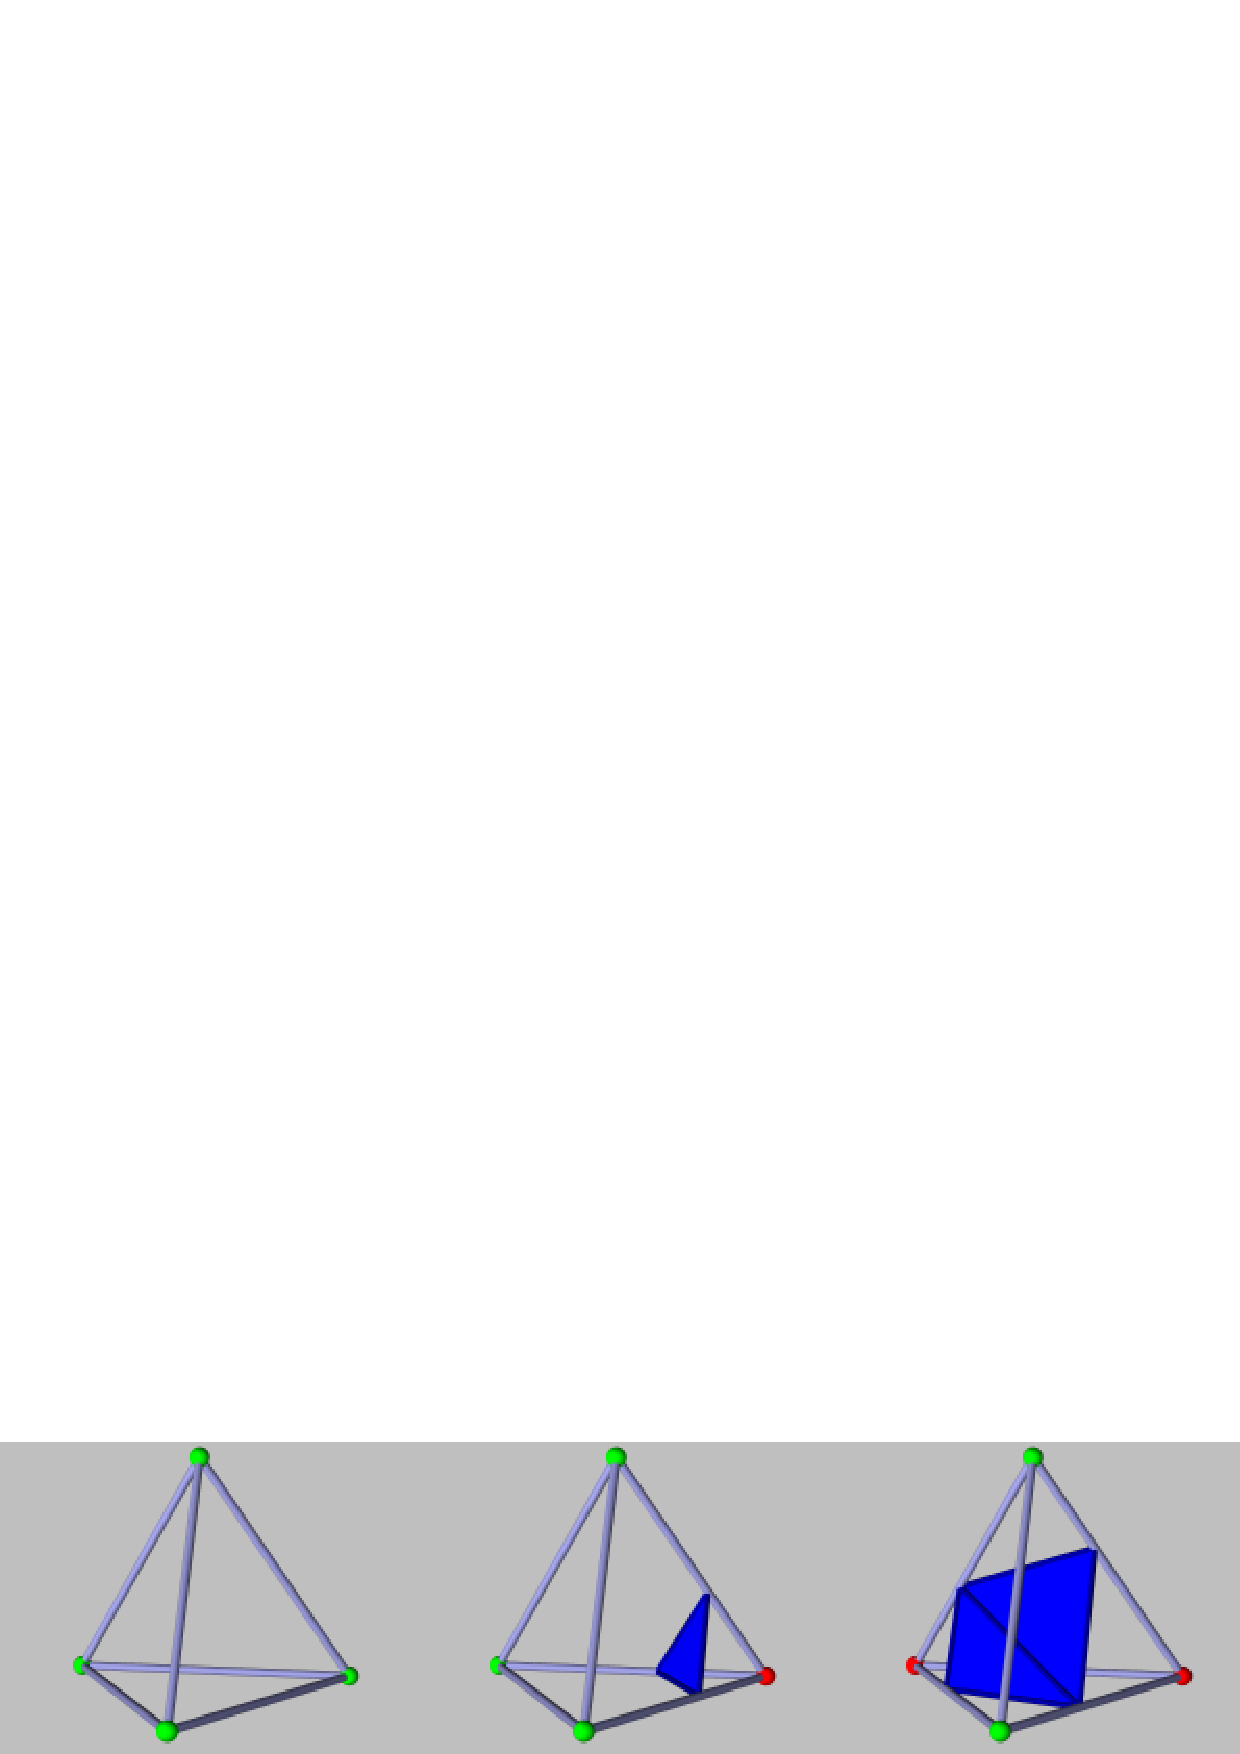
\includegraphics[width=.8\textwidth]{Skin_surface_3/marching}
\end{center}
\end{ccTexOnly}
\begin{ccHtmlOnly}
<CENTER>
<img border=0 src="./marching.png"
alt="Cases of the marching tetrahedra algorithm.">
</CENTER>
\end{ccHtmlOnly}

\caption{\label{SkinSurface3-fig-marching} Cases of the marching
  tetrahedra algorithm.}
\end{figure}

Our implementation takes four arguments: the input triangulation, the
surface mesh, a policy class and an observer class.  The algorithm is
performed on the triangulation and the resulting mesh is stored in the
polyhedron. The \ccc{CGAL::Polyhedron_incremental_builder_3} is used
for constructing the polyhedron.

The policy class defines a predicate and a constructor. The predicate
is able to test whether a vertex of the triangulation lies inside or
outside the surface and the constructor is able to return the
intersection point of the surface with an edge of the triangulation
whose vertices lie on opposite sides of the surface. For skin surfaces
the intersection point is unique.

The observer class implements two functions that are called after the
construction of a vertex and a facet of the polyhedron. After
insertion of a vertex in the polyhedron a function is called with the
vertex of the polyhedron and the corresponding edge of the
triangulation. Similarly, after insertion of a facet in the polyhedron
a function is called with the facet of the polyhedron and the
corresponding cell of the triangulation. 

